\documentclass[10pt]{article}
\usepackage[utf8]{inputenc}
\usepackage[T1]{fontenc}
\usepackage[margin=2cm]{geometry}
\usepackage{graphicx,booktabs,float,amsmath,amssymb,textcomp,xcolor}
\usepackage{listings}
\usepackage[hidelinks]{hyperref}
\lstset{basicstyle=\ttfamily\small,breaklines=true,frame=single,columns=fullflexible,keepspaces=true}
\setlength{\parskip}{0.5em}\setlength{\parindent}{0pt}
\title{Report 1: CUDA Programmatic Dependent Launch for a MegaFold Training Step on one GH200}
\author{MegaFold PDL investigation --- NCSA DeltaAI, 1$\times$ NVIDIA GH200}
\date{November 2026}
\begin{document}
\maketitle

\textbf{Bottom line.} I added PDL to every hand-written MegaFold Triton kernel and to all Triton code that \texttt{torch.compile} generates, made it correct under \texttt{torch.compile}, and measured it against the baseline on one GH200. \textbf{End-to-end, PDL makes no measurable difference}: every PDL variant falls inside the run-to-run noise of the baseline (paired step-time ratio 0.989--0.995, all 95\% CIs include 1.0; two identical baseline runs differ by 0.991). The step is \textbf{CPU/launch-bound} (GPU idle $\approx$64\% of a traced step, \textasciitilde{}168k GPU ops/step), and only \textbf{3.6\% of adjacent kernel pairs} are PDL-eligible, so PDL can affect $\lesssim$1\% of the step even in the best case. At kernel level, a naive placement of the PDL trigger \emph{costs} 3.7\%; the best placement gains +0.3\%.


\begin{table}[H]\centering\small
\resizebox{\ifdim\width>\textwidth\textwidth\else\width\fi}{!}{%
\begin{tabular}{llllll}
\toprule
 & step time, median (s) & paired ratio vs baseline (95\% CI) & first step incl. compile (s) & peak mem (GiB) & loss parity \\
\midrule
\textbf{Baseline} (primary run, 20 timed steps) & \textbf{8.93} (mean 9.02, $\sigma$ 0.94, min 7.46) & --- & 129.7 & 40.15 & --- \\
Baseline, interleaved reps 1 / 2 & 9.81 / 9.70 & rep2/rep1: \textbf{0.991} [0.976, 1.005] $\leftarrow$ noise floor & 130.2 / 129.2 & 40.15 & --- \\
PDL, all kernels, early trigger & 9.72 / 9.70 & 0.989 [0.980, 1.001] & 136.5 / 135.0 & 40.15 & \checkmark{} \\
PDL, all kernels, implicit trigger & 9.56 / 9.72 & 0.9935 [0.979, 1.001] & 134.7 / 135.6 & 40.15 & \checkmark{} \\
PDL, tiled kernels only & 9.55 / 10.33 & 0.995 [0.987, 1.052] & 138.1 / 140.9 & 40.15 & \checkmark{} \\
\bottomrule
\end{tabular}}
\end{table}

\emph{Paired ratio:} every step index uses an identical RNG stream in every variant (the per-step work varies with the step's random draws), so each PDL step is divided by the same step of the baseline run from the same interleaved repetition; 2 reps $\times$ 10 steps = 20 ratios; bootstrap CI of the median.


\begin{figure}[H]\centering
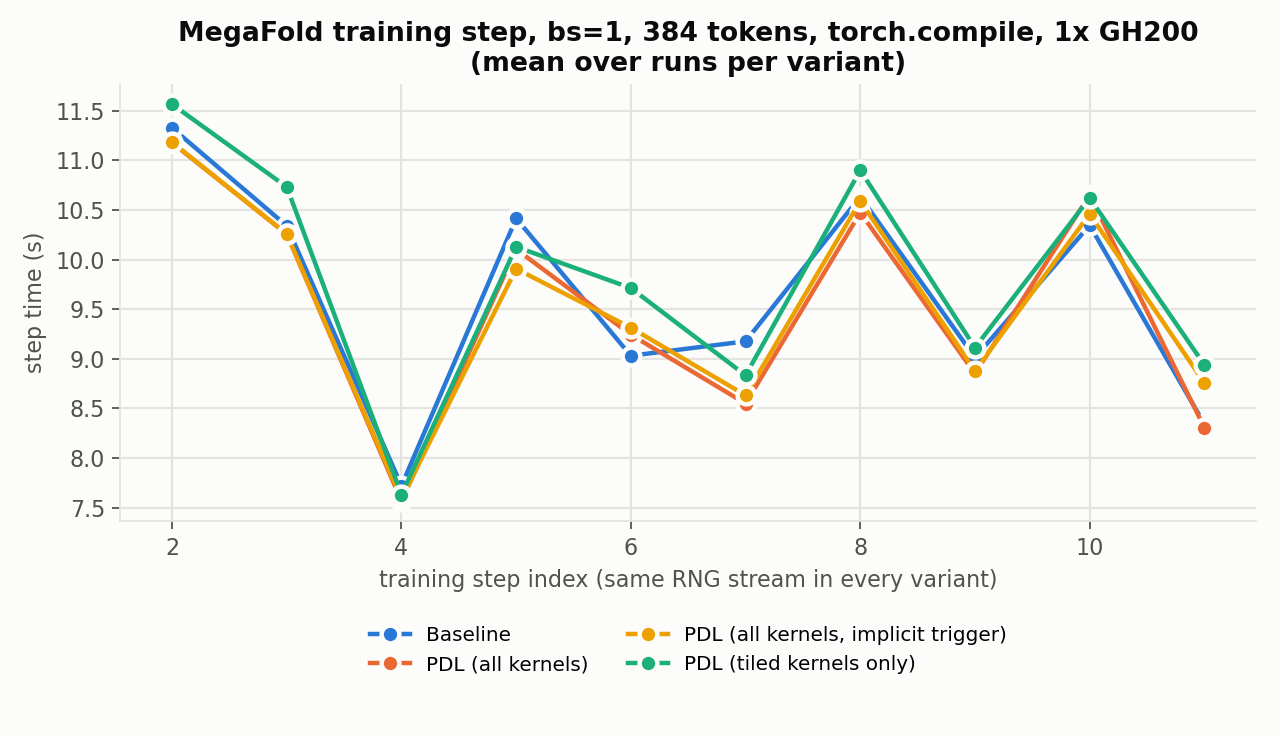
\includegraphics[width=\linewidth]{figures/e2e_step_time.png}
\caption{per-step time}
\end{figure}


\section{Setup}

\begin{table}[H]\centering\small
\resizebox{\ifdim\width>\textwidth\textwidth\else\width\fi}{!}{%
\begin{tabular}{ll}
\toprule
 &  \\
\midrule
Hardware & NCSA DeltaAI, 1$\times$ NVIDIA GH200 120GB (H100-class sm\_90, 96 GB HBM3 visible), Grace CPU, driver 595.71 \\
Software & PyTorch 2.10.0+cu129, Triton 3.6.0, CUDA 12.9, Python 3.12 (\texttt{python/miniforge3\_pytorch/2.10.0}) \\
Model & MegaFold AlphaFold3, \texttt{configs/megafold\_1x1.yaml} (\texttt{use\_optimized\_evo: triton}, 48-block Pairformer, activation checkpointing as configured), 509,004,585 parameters \\
MegaFold kernels & EvoFlash-3D attention, fused LayerNorm-Linear and fused SwiGLU Transition all active (nsys: \textasciitilde{}2.9k / 6.7k / 1.9k launches per step) \\
Input & batch size 1, \textbf{384 tokens} (single protein chain, 3,481 atoms), MSA depth 512, 4 templates --- fixed synthetic example collated by MegaFold's own \texttt{collate\_inputs\_to\_batched\_atom\_input} (the PDB data / MSA caches are not on the system; the step's compute is shape-, not value-dependent) \\
Training step & exactly what \texttt{megafold/trainer.py} does per step: \texttt{loss = model(**batch, dtype=bf16, return\_loss\_breakdown=True, call\_confidence\_head=False)}, \texttt{loss.backward()}, \texttt{clip\_grad\_norm\_(10)}, \texttt{Adam(lr=1e-4).step()}, \texttt{zero\_grad()} (DeepSpeed ZeRO-0 in the 1x1 config is equivalent) \\
Compile & \texttt{torch.compile(model, dynamic=False)}, \textbf{\texttt{TORCH\_COMPILE\_DEBUG=1}} for every run, cold Triton/Inductor caches per run \\
Method & \texttt{benchmarks/train\_step\_bench.py}; wall time per step with \texttt{cuda.synchronize()}; warm-up steps excluded; variants interleaved on one node \\
\bottomrule
\end{tabular}}
\end{table}

\textbf{Changes required to run the 1x1 training step under \texttt{torch.compile} at all} (applied to \emph{both} baseline and PDL; MegaFold ships \texttt{use\_torch\_compile=False}, so this path had never been exercised):


\begin{enumerate}
\item \texttt{megafold/model/FusedTransition/fused\_transition.py} --- the SwiGLU backward wrote the gradient \emph{in place into the saved forward input} and returned it. aot-autograd forbids in-place mutation of a view produced by another custom \texttt{autograd.Function}. The kernel now writes \texttt{dx} into a fresh buffer (same bytes read/written as before).
\item \texttt{megafold/distributed/comm.py} --- \texttt{scatter}/\texttt{gather} are the identity when there is one sequence-parallel rank; they now return the input directly instead of routing it through a custom \texttt{autograd.Function} (returning an input from a Function creates an alias torch.compile rejects).
\item Harness: \texttt{dynamic=False} (Dynamo 2.10 crashes tracing MegaFold's Triton launches once a dimension becomes symbolic: \texttt{SymNodeVariable has no attribute value}), and \texttt{CXX=g++} (DeltaAI's PrgEnv sets \texttt{CXX=CC}, the Cray wrapper, which breaks Inductor's C++ codegen).
\end{enumerate}

\section{Baseline}

Primary baseline (cold caches, 3 warm-up + 20 timed steps): \textbf{median 8.93 s/step} (mean 9.02 s, $\sigma$ 0.94 s, min 7.46 s); first step including compilation 129.7 s; peak allocated memory 40.15 GiB. The $\pm$10\% step-to-step spread is \emph{deterministic} (it reproduces step-for-step across runs): it comes from the per-step random draws of AF3 training (e.g. the number of recycling iterations), which is why all comparisons are paired by step index. Separately, whole runs drift by up to \textasciitilde{}3\% on the shared node, which is why variants are interleaved.


\section{Where and how PDL was applied}

PDL (Hopper+, \texttt{cudaLaunchAttributeProgrammaticStreamSerialization}) lets kernel \emph{N+1} on a stream be \textbf{launched while kernel \emph{N} is still running}. \emph{N+1}'s CTAs are scheduled once every CTA of \emph{N} has executed \texttt{griddepcontrol.launch\_dependents} (or exited); they run their prologue and block in \texttt{griddepcontrol.wait} until \emph{N} has fully completed and flushed memory. It hides launch latency and the predecessor's tail; it does not reduce the number of launches or their CPU cost.


\subsection{MegaFold's hand-written Triton kernels (all 10)}

Mechanism (\texttt{megafold/model/pdl.py}): a global \texttt{tl.constexpr} gate and a \texttt{@triton.jit} prologue called as the \textbf{first statement} of every kernel, plus \texttt{launch\_pdl=} at every launch site (12 sites):


\begin{lstlisting}
@triton.jit
def pdl_prologue():
    if USE_PDL:                                  # constexpr: compiled out when MEGAFOLD_PDL is unset
        tl.extra.cuda.gdc_wait()                 # griddepcontrol.wait  - before ANY global load/store
        if EARLY_TRIGGER:
            tl.extra.cuda.gdc_launch_dependents()  # griddepcontrol.launch_dependents

_attn_fwd[grid](..., launch_pdl=LAUNCH_PDL)      # cudaLaunchKernelEx + programmatic serialization
\end{lstlisting}

\begin{table}[H]\centering\small
\resizebox{\ifdim\width>\textwidth\textwidth\else\width\fi}{!}{%
\begin{tabular}{lllll}
\toprule
kernel & file & role & grid (n = 384) & class \\
\midrule
\texttt{\_attn\_fwd} & \texttt{FusedEvoAttention/evoattention.py} & EvoFlash-3D attention forward & (n/16, b$\cdot$s$\cdot$h) tiles & tiled \\
\texttt{\_attn\_bwd\_preprocess} & \textquotedbl{} & D = rowsum(dO$\circ$O) & (n/32, b$\cdot$s$\cdot$h) & tiled \\
\texttt{\_attn\_bwd\_dk\_dv} & \textquotedbl{} & dK, dV (+ d pair-bias, atomics) & (n/64, b$\cdot$s$\cdot$h) & tiled \\
\texttt{\_attn\_bwd\_dq} & \textquotedbl{} & dQ & (n/16, b$\cdot$s$\cdot$h) & tiled \\
\texttt{\_second\_forward\_kernel} & \texttt{FusedLayernormLinear/fused\_layernorm\_linear.py} & normalize + matmul & M/BM $\cdot$ N/BN tiles & tiled \\
\texttt{\_first\_backward\_kernel} & \textquotedbl{} & dY$\cdot$W$^{T}$, dW (atomics) & M/BM $\cdot$ K/BK tiles & tiled \\
\texttt{\_first\_forward\_kernel} & \textquotedbl{} & LayerNorm mean / rstd & \textbf{(M,)}, one row per CTA, M = n$^2$ = 147,456 & row-wise \\
\texttt{\_second\_backward\_kernel} & \textquotedbl{} & LayerNorm dX & \textbf{(M,)} & row-wise \\
\texttt{\_swiglu\_forward\_kernel} & \texttt{FusedTransition/fused\_transition.py} & silu(b)$\cdot$a & \textbf{(M,)} & row-wise \\
\texttt{\_swiglu\_backward\_kernel} & \textquotedbl{} & d(a, b) & \textbf{(M,)} & row-wise \\
\bottomrule
\end{tabular}}
\end{table}

\textbf{Why it is safe.} \texttt{gdc\_wait} precedes every global memory access, so a kernel can never read data its predecessor has not finished writing (RAW) nor overwrite data the predecessor still reads (WAR). The early trigger only affects \emph{scheduling}: a dependent's \texttt{gdc\_wait} always waits for full completion. Kernels not launched with PDL keep normal stream ordering. Verified: forward outputs and loss are bitwise identical to the baseline; gradients differ only at the level of the baseline's own run-to-run noise (the LayerNorm-Linear and attention backward accumulate with float atomics, so even two baseline runs are not bitwise identical) --- \texttt{results/kernels\_compare*.json}. PTX check: \texttt{griddepcontrol} appears in 0/10 baseline kernels and 10/10 PDL kernels (\texttt{results/ptx\_griddepcontrol.txt}).


Policy knobs (all read at import): \texttt{MEGAFOLD\_PDL=1} enables; \texttt{MEGAFOLD\_PDL\_KERNELS=all|tiled}; \texttt{MEGAFOLD\_PDL\_TRIGGER=early|implicit} (implicit = no explicit trigger; dependents are released as CTAs exit); \texttt{MEGAFOLD\_PDL\_LAUNCH=0} (diagnostic: instructions compiled in, normal launch).


\subsection{Kernels generated by \texttt{torch.compile} (Inductor)}

\texttt{torch.\_inductor.config.triton.enable\_pdl = True} makes Inductor insert \texttt{gdc\_wait()} before the first load and \texttt{gdc\_launch\_dependents()} after the last load of every generated Triton kernel and launch them with \texttt{launch\_pdl}. In each PDL run 135 of 153 compiled graphs contain PDL code (\textasciitilde{}448 \texttt{gdc\_wait} sites, \textasciitilde{}462 kernels launched with \texttt{launch\_pdl=True}); the baseline has none.


\subsection{Two bugs that had to be fixed for PDL to work at all}

\begin{enumerate}
\item \textbf{Inductor PDL codegen crash} (PyTorch 2.10): \texttt{\_handle\_pdl\_after\_load} calls \texttt{cse.generate(...)} without \texttt{shape=}, so every kernel with a load fails with \texttt{AssertionError: TritonCSEVariable must have shape}. Fixed in the harness by passing \texttt{shape=()} (the generated value is the scalar \texttt{0}).
\item \textbf{Silent NaN loss --- PDL instructions break Inductor's mutation analysis.} Under \texttt{torch.compile}, Dynamo traces MegaFold's Triton launches into the graph (\texttt{triton\_kernel\_wrapper\_functional}), and Inductor statically analyses each kernel's TTIR to learn which pointers it writes. A non-pure \texttt{tt.elementwise\_inline\_asm} --- which \texttt{gdc\_wait}/\texttt{gdc\_launch\_dependents} are, by necessity --- makes that analysis bail out to "every input is mutated", and on this model that fallback produced uninitialised outputs (NaN loss from step 0, \textbf{even with PDL launches disabled}). Isolated, the same kernels are correct, which is why the kernel-level check did not catch it. Diagnosis: a NaN tracer on the fused \texttt{autograd.Function}s pinpointed SwiGLU/LayerNorm-Linear calls returning non-finite outputs from finite inputs; the FX graphs showed \texttt{x\_ptr}/\texttt{X\_ptr} newly in \texttt{tensors\_to\_clone}. Fix (\texttt{megafold/model/pdl.py}): before the analysis, drop inline-asm ops that have \textbf{no operands} (they receive no pointer, so they cannot mutate a parameter). Inductor then infers exactly the baseline's mutation sets (\texttt{results/mutation\_analysis\_check.txt}) and the loss matches the baseline. All PDL end-to-end numbers measured before this fix were invalid and are kept only as evidence in \texttt{results/invalid\_nan\_before\_fix/}.
\end{enumerate}

\section{Profiles of the training step (nsys, one steady-state step per run)}

Each figure: top --- every GPU op of one training step (blank = GPU idle); bottom --- a 3 ms window at the same logical point in every run, with ops that start before their predecessor ends drawn on the upper lane (only possible with PDL). nsys inflates the step (\textasciitilde{}9 s $\rightarrow$ \textasciitilde{}13 s) because \textasciitilde{}168k ops are recorded; proportions, not absolute times, are the point. Raw traces: \texttt{results/**/nsys/*.nsys-rep}.


\begin{table}[H]\centering\small
\resizebox{\ifdim\width>\textwidth\textwidth\else\width\fi}{!}{%
\begin{tabular}{lllllllllllll}
\toprule
run & GPU ops & traced step (s) & GPU busy (s) & GPU idle & median gap (\textmu{}s) & PDL overlaps (count / total ms) & EvoFlash-3D (s) & LayerNorm-Linear (s) & SwiGLU (s) & Inductor (s) & GEMM (s) & ATen eager (s) \\
\midrule
Baseline & 168,410 & 13.36 & 4.819 & 8.54 s (64\%) & 13.7 & 0 / 0.0 & 0.918 & 0.799 & 0.075 & 0.027 & 0.731 & 2.246 \\
PDL, all kernels, early trigger & 168,410 & 15.67 & 5.218 & 10.45 s (67\%) & 20.9 & 4,339 / 18.7 & 0.922 & 1.193 & 0.099 & 0.028 & 0.730 & 2.244 \\
PDL, all kernels, implicit trigger & 168,410 & 15.96 & 4.824 & 11.13 s (70\%) & 23.3 & 2,959 / 0.7 & 0.923 & 0.801 & 0.075 & 0.028 & 0.730 & 2.246 \\
PDL, tiled kernels only & 168,410 & 15.95 & 4.825 & 11.12 s (70\%) & 24.1 & 2,180 / 1.7 & 0.925 & 0.801 & 0.075 & 0.028 & 0.730 & 2.245 \\
\bottomrule
\end{tabular}}
\end{table}

The op sequence is identical in every run (168,410 ops). PDL produces thousands of real overlaps, but they total at most 18.7 ms of a \textasciitilde{}13--16 s traced step. With the early trigger, GPU busy time \emph{rises} by 0.4 s --- almost entirely LayerNorm-Linear (+0.39 s) and SwiGLU (+0.02 s), whose row-wise kernels pay the per-CTA trigger cost; Inductor, GEMM and ATen time are unchanged. With the implicit trigger or tiled-only policy, busy time equals the baseline's to within 6 ms. The traced span differences (13.4 s vs \textasciitilde{}15.9 s) are idle time, i.e. CPU-side; they vary between nsys sessions and are not a PDL effect (the untraced, interleaved measurements in the summary table show no difference).



\textbf{Baseline}

\begin{figure}[H]\centering
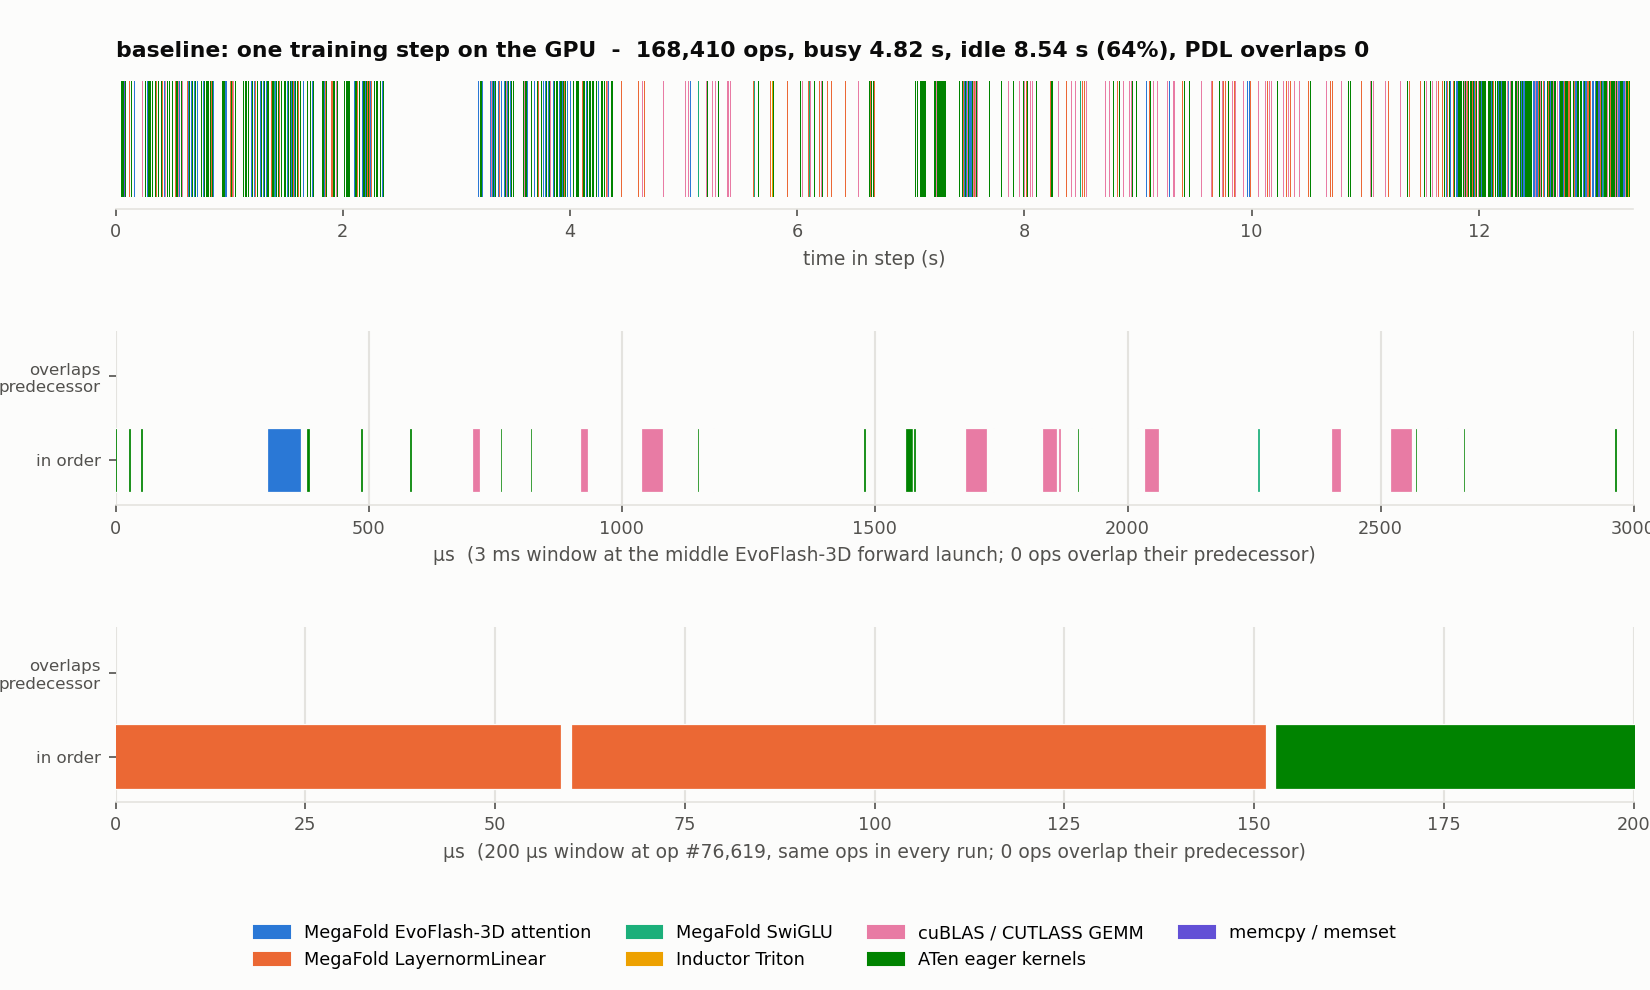
\includegraphics[width=\linewidth]{figures/profile_baseline.png}
\caption{baseline profile}
\end{figure}

\textbf{PDL, all kernels, early trigger}

\begin{figure}[H]\centering
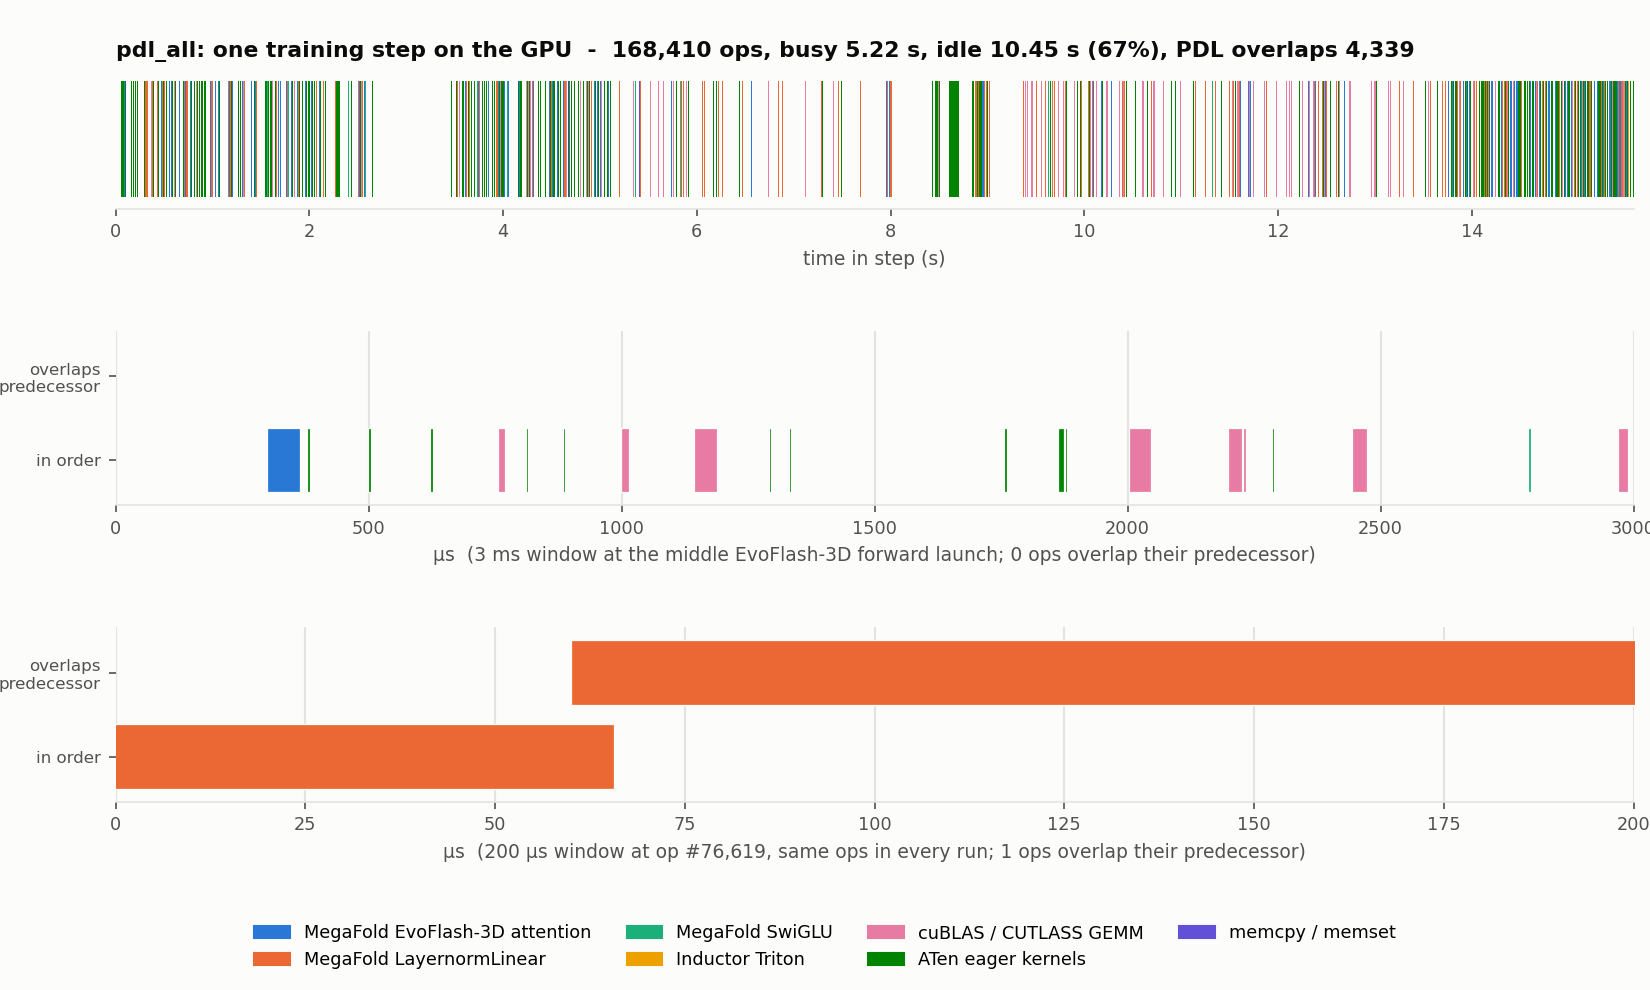
\includegraphics[width=\linewidth]{figures/profile_pdl_all.png}
\caption{pdl all profile}
\end{figure}

\textbf{PDL, all kernels, implicit trigger}

\begin{figure}[H]\centering
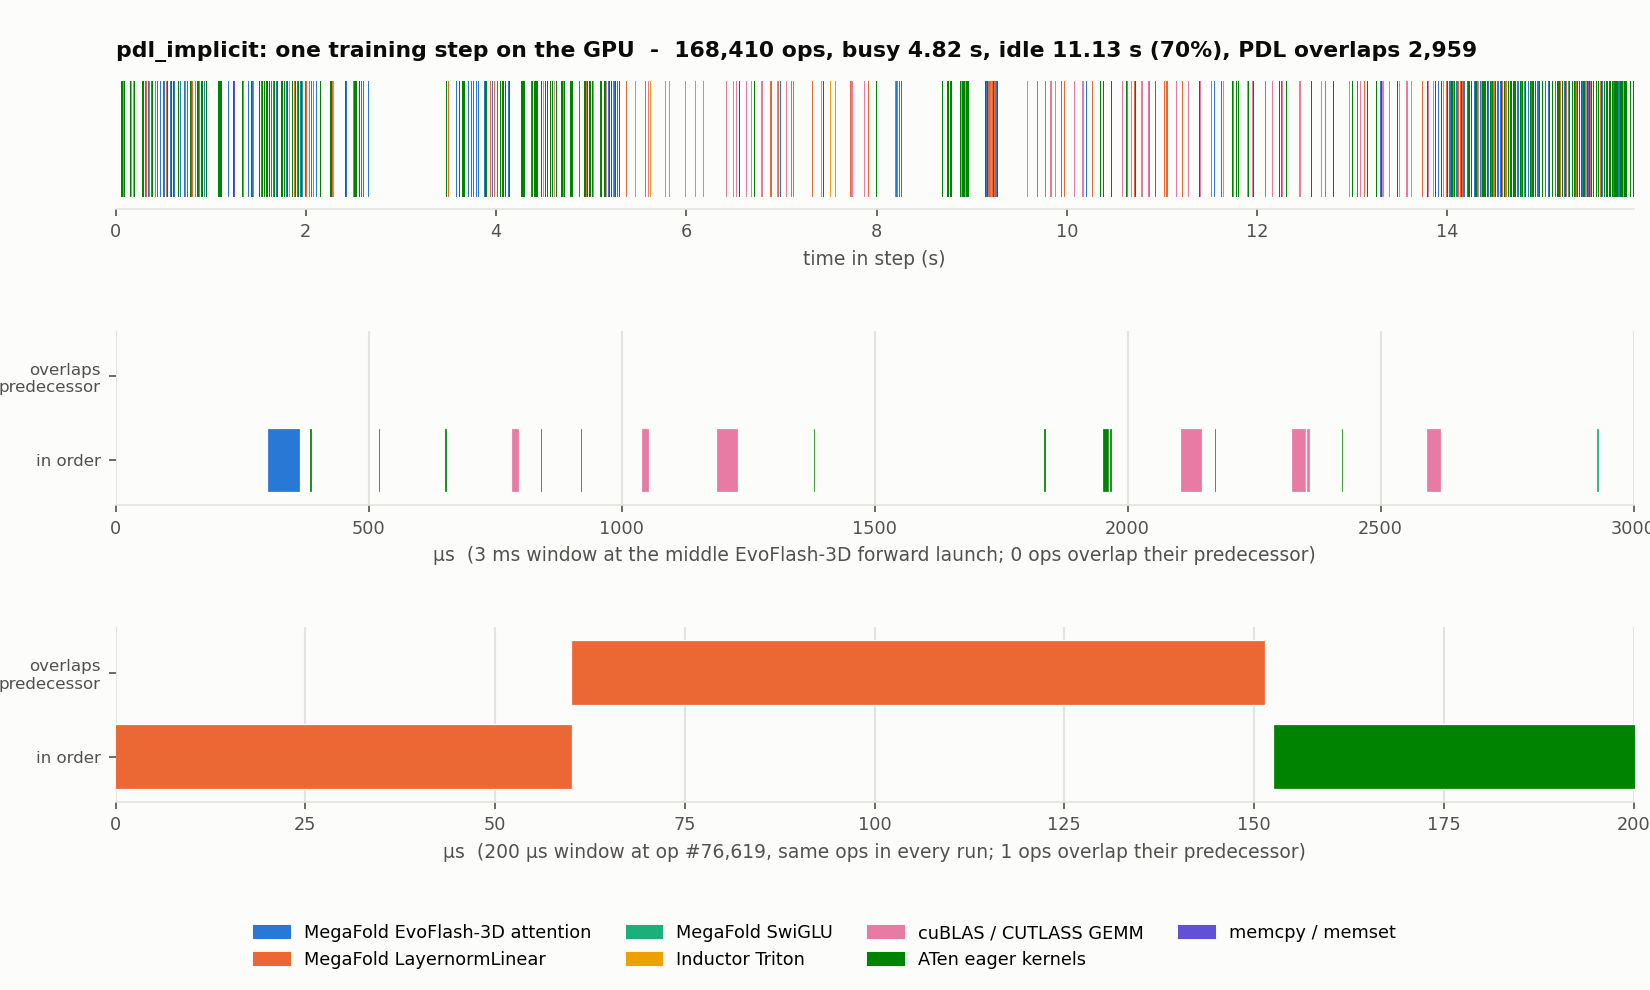
\includegraphics[width=\linewidth]{figures/profile_pdl_implicit.png}
\caption{pdl implicit profile}
\end{figure}

\textbf{PDL, tiled kernels only}

\begin{figure}[H]\centering
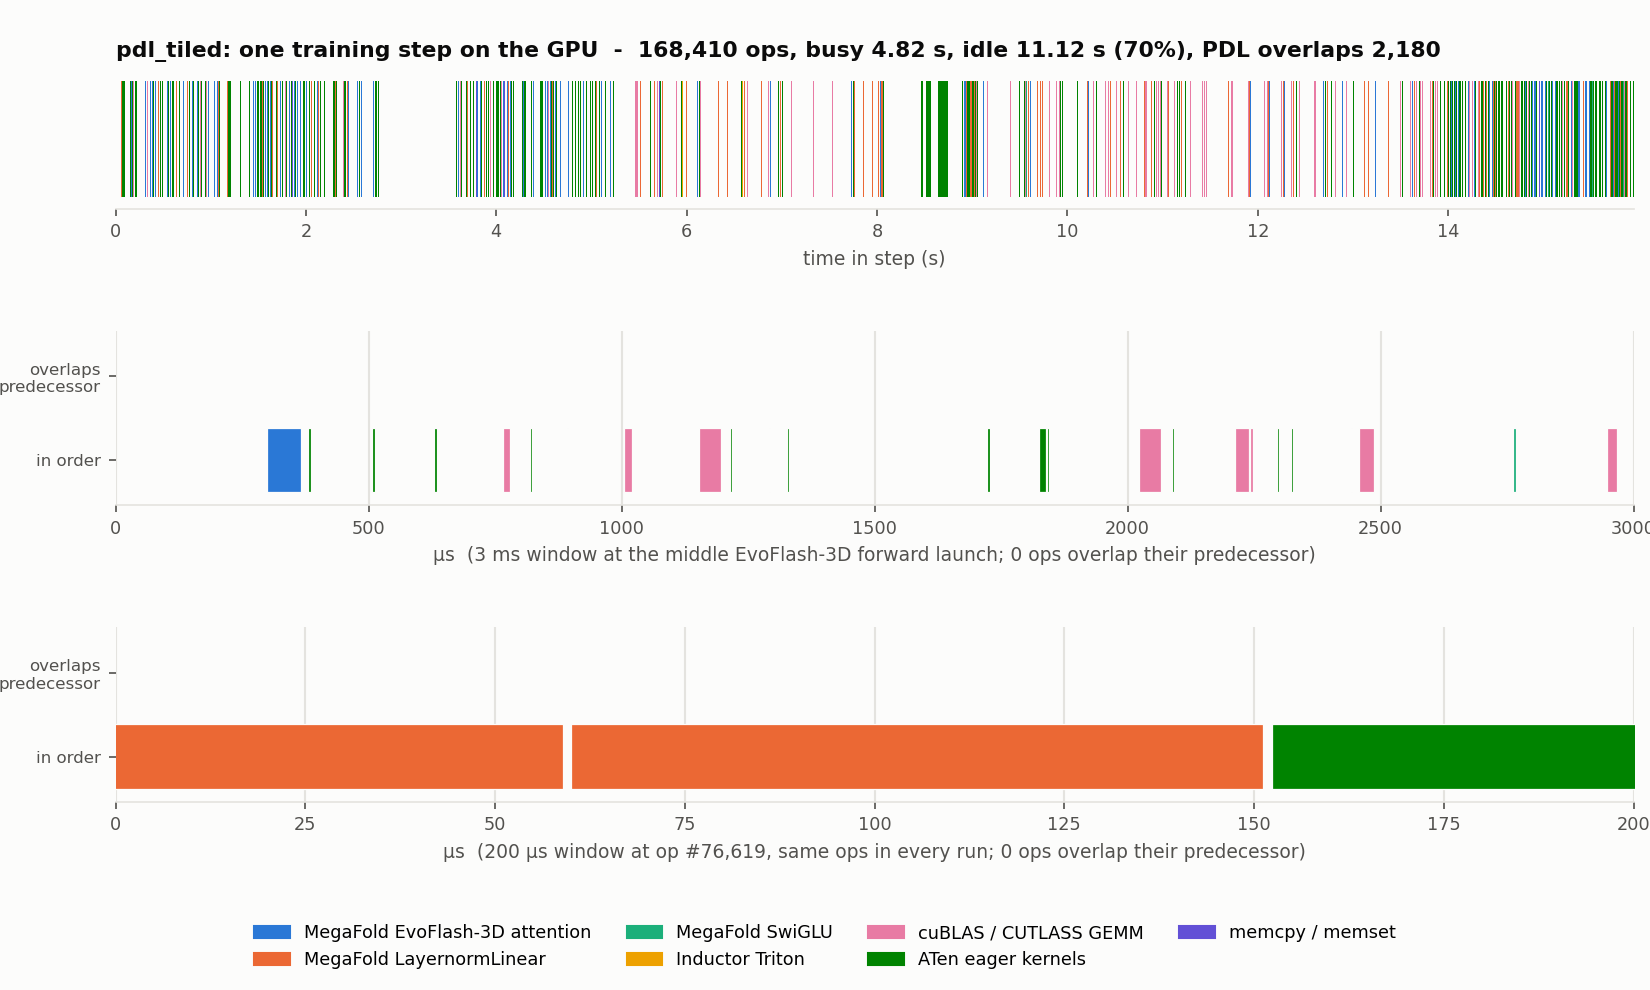
\includegraphics[width=\linewidth]{figures/profile_pdl_tiled.png}
\caption{pdl tiled profile}
\end{figure}

Where the baseline step goes:


\begin{figure}[H]\centering
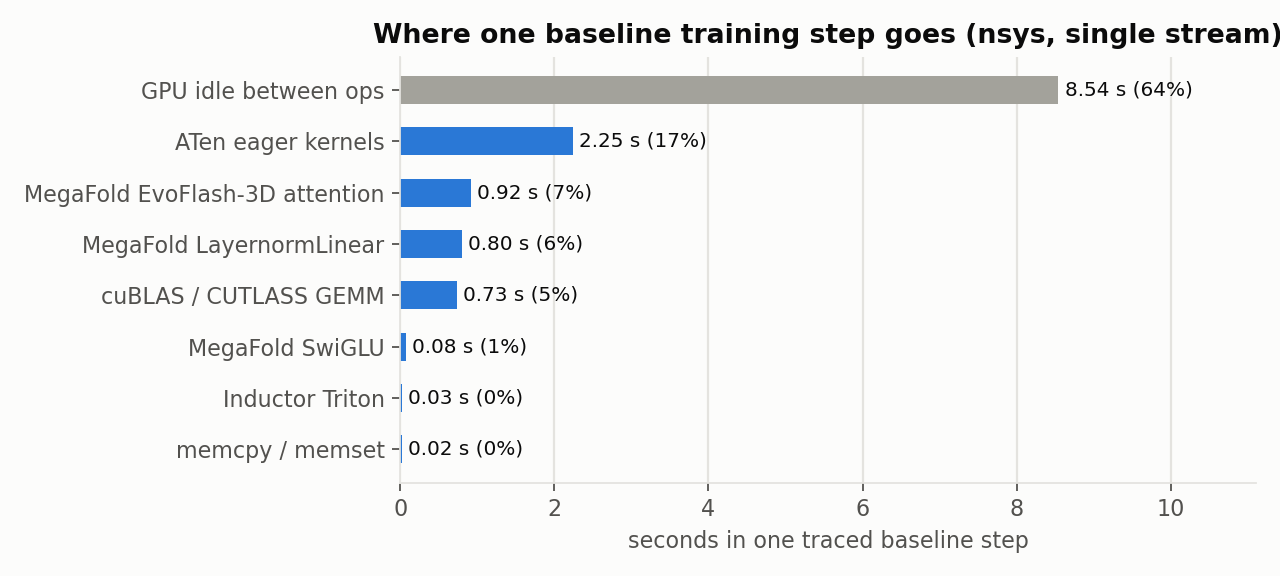
\includegraphics[width=\linewidth]{figures/baseline_step_breakdown.png}
\caption{baseline breakdown}
\end{figure}

\section{Why PDL cannot pay off here}

From the baseline trace (\texttt{results/baseline/nsys/}):


\begin{itemize}
\item \textbf{The step is CPU/launch-bound.} 168,410 GPU ops per step; the GPU is idle 64\% of the traced
\end{itemize}
step (untraced: 9.1 s wall vs 4.8 s of GPU work). The median inter-op gap (13.7 \textmu{}s, p90 101 \textmu{}s, p99 306 \textmu{}s) is the CPU not having issued the next op yet. PDL can only overlap a kernel that is already queued behind its predecessor.

\begin{itemize}
\item \textbf{Almost nothing is PDL-eligible.} PDL needs \emph{both} neighbours to be PDL-aware Triton kernels.
\end{itemize}
65\% of ops are eager ATen kernels (\texttt{vectorized\_elementwise\_kernel} etc. --- \texttt{torch.compile} leaves most of the model eager because of graph breaks: only 2,660 Inductor kernels per step, 1.6\%), plus 35k cuBLAS/CUTLASS GEMMs. Only \textbf{6,035 of 168,409 adjacent pairs (3.6\%)} are Triton$\rightarrow$Triton.

\begin{itemize}
\item \textbf{The eligible pairs are already back-to-back}: median gap 1.2 \textmu{}s, 110 ms of the 8,541 ms of total
\end{itemize}
gap time. That is the ceiling for PDL on this step: $\lesssim$1\%.


\section{Kernel-level analysis: the trigger placement matters}

Eager stack of 8 pairformer-shaped blocks (LayerNorm-Linear $\rightarrow$ EvoFlash-3D triangle attention $\rightarrow$ SwiGLU Transition, n = 384, d = 128), forward + backward, median of 20 (\texttt{benchmarks/pdl\_kernel\_check.py}):


\begin{table}[H]\centering\small
\resizebox{\ifdim\width>\textwidth\textwidth\else\width\fi}{!}{%
\begin{tabular}{lll}
\toprule
variant & ms & vs baseline 46.81 ms \\
\midrule
PDL, all kernels, early trigger & 48.61 & \textbf{$-$3.7\%} \\
PDL instructions only, normal launch & 48.73 & $-$3.9\% \\
PDL, all kernels, implicit trigger & 46.66 & \textbf{+0.3\%} \\
PDL, tiled kernels only & 46.79 & $\pm$0.0\% \\
\bottomrule
\end{tabular}}
\end{table}

\begin{figure}[H]\centering
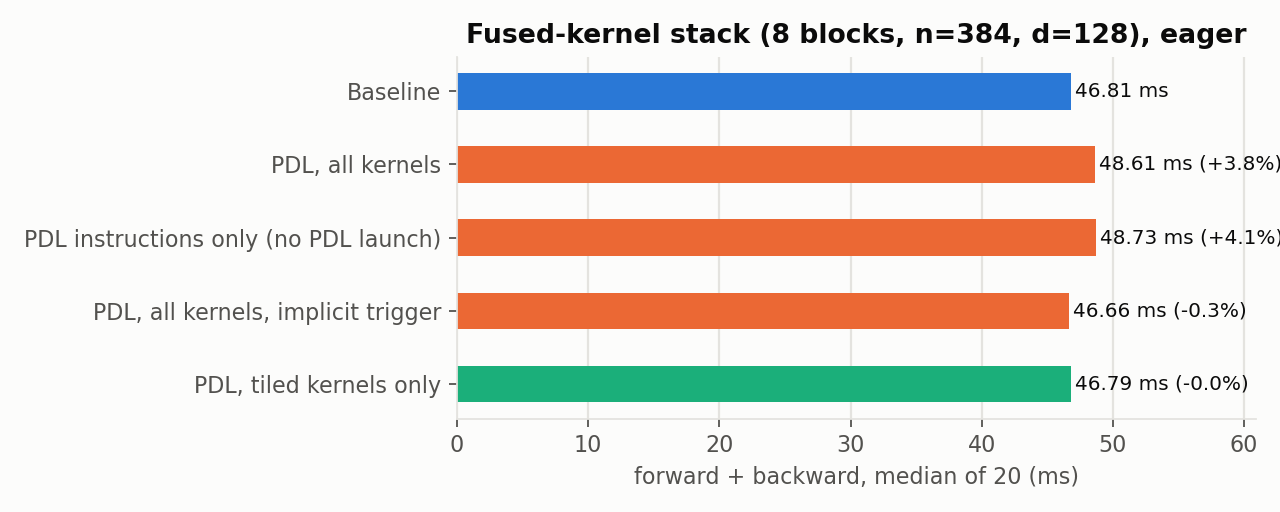
\includegraphics[width=\linewidth]{figures/kernel_variants.png}
\caption{kernel variants}
\end{figure}

The PDL overlap itself works (320 kernel overlaps per 5 iterations in nsys, idle between kernels down from 4.56 to 3.93 ms), but in the early-trigger variant the \textbf{row-wise kernels get much slower}: \texttt{\_first\_forward\_kernel} +89\%, \texttt{\_second\_backward\_kernel} +187\%, \texttt{\_swiglu\_forward\_kernel} +43\%; tiled kernels are within 0--2.5\%. The "instructions only" variant is just as slow, so the cost is \textbf{executing \texttt{griddepcontrol.launch\_dependents} in each of \textasciitilde{}147k tiny CTAs}, not the scheduling; with the implicit trigger (\texttt{gdc\_wait} only) the penalty disappears. Lesson: on kernels with many short CTAs, do not trigger explicitly --- let CTA exit release the dependent.


\begin{figure}[H]\centering
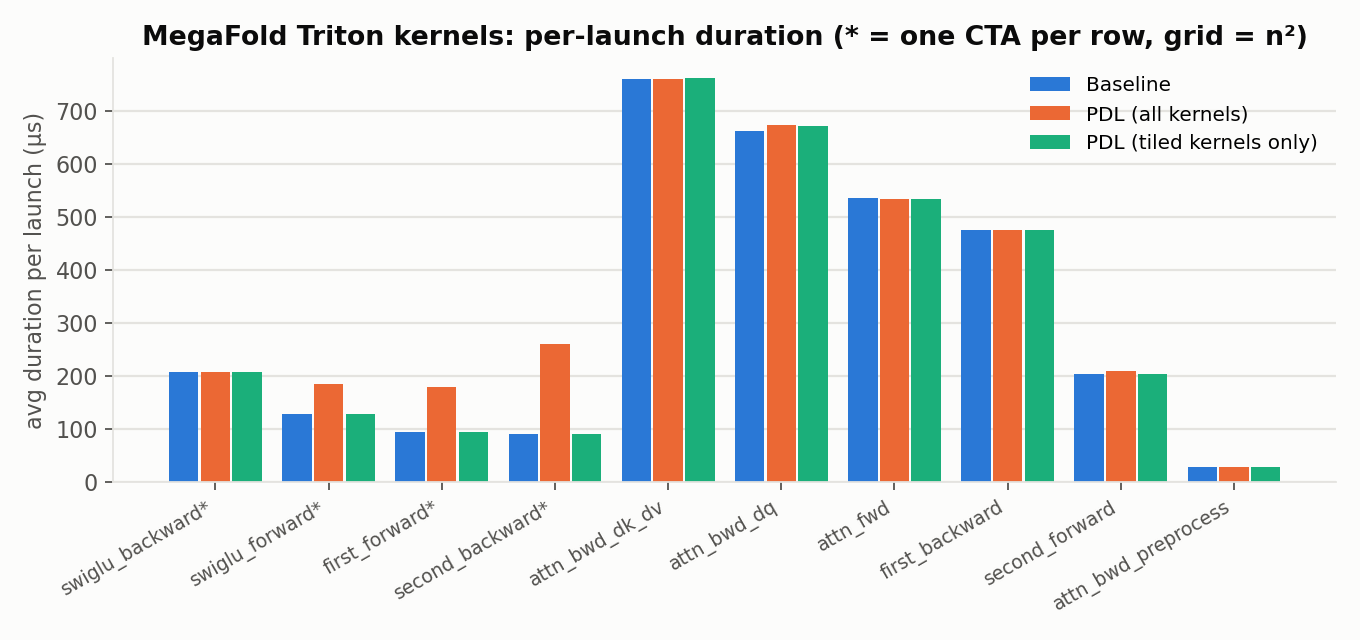
\includegraphics[width=\linewidth]{figures/per_kernel_duration.png}
\caption{per-kernel durations}
\end{figure}

\section{Caveats}

\begin{itemize}
\item Synthetic input (no PDB data / MSA caches on the system); the compute graph and shapes match a
\end{itemize}
384-token crop, values do not affect kernel timing, and identical inputs make variants comparable.

\begin{itemize}
\item \texttt{call\_confidence\_head=False} for every step (the trainer calls it every 10th step).
\item nsys adds \textasciitilde{}45\% to the step; the gap/eligibility figures are proportions of a traced step.
\item The \textasciitilde{}1\% median differences end-to-end are within run-to-run noise; resolving effects of that size
\end{itemize}
would need many more interleaved repetitions than one 2-hour allocation allows.


\section{Reproduce}

\begin{lstlisting}
# environment (DeltaAI): module load python/miniforge3_pytorch/2.10.0; conda activate base;
#   python -m venv --system-site-packages ~/venvs/megafold; pip install -r requirements (see README)
sbatch scripts/hold_node.sh                       # holds one GH200 (ghx4-interactive, 2 h)
srun --jobid=<id> --overlap -n1 bash scripts/run_investigation.sh   # kernel-level variants
srun --jobid=<id> --overlap -n1 bash scripts/run_e2e_final.sh       # interleaved e2e + nsys
python benchmarks/make_report.py; python benchmarks/plot_profiles.py name=<trace.csv> ...
\end{lstlisting}
Baseline runs use a checkout of the \textbf{\texttt{baseline} branch} of this repository (original MegaFold kernels plus the two compile fixes; measured at commit \texttt{0c97c88}, harness additions in \texttt{a890b55}), passed as \texttt{BASE\_TREE}. PDL runs use the \texttt{main} branch with \texttt{MEGAFOLD\_PDL=1} (Report 1 measurements: commit \texttt{bc7e216}).

\end{document}
